\subsection{Implementasi Halaman \textit{Login}}
Halaman ini dapat diakses oleh semua pengguna, baik yang belum terdaftar maupun sudah, dengan pengecualian pengguna tidak dalam keadaan sudah \textit{login}. Halaman ini menampilkan \textit{form} berisi elemen \textit{input} \textit{email} dan \textit{password}, dan tombol \textit{login}. Kasus normal dan alternatif dapat dilihat pada Tabel \ref{uc01.02}. Tidak ada \textit{view logic} dalam halaman ini. Kode sumber implementasi \textit{back-end} dapat dilihat pada Kode Sumber \ref{cdbe.01-02}.

\begin{figure}[H]
	\centering
	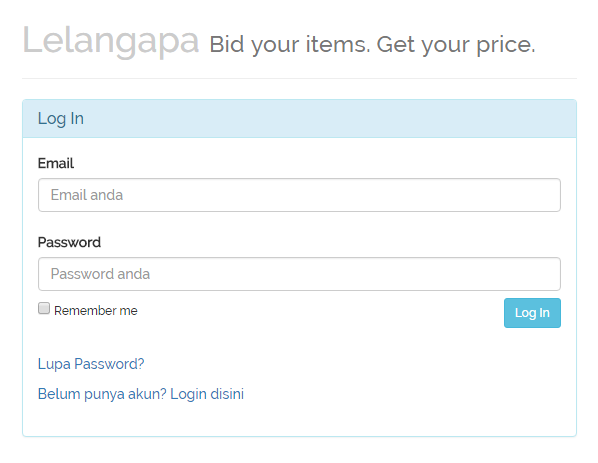
\includegraphics[width=.8\textwidth]{images/bab4/ui/01-02.png}
	\caption{Halaman Antarmuka \textit{Login}}
	\label{ui.01-02}
\end{figure}

\begin{lstlisting}[label=cdbe.01-02,style=php,caption=Implementasi Antarmuka \textit{Login}]
public function showLoginForm(){
	/*Menampilkan halaman login; Method : GET */
	return view('auth.login2');
}
public function login(Request $request){
	/* Setelah klik tombol login
	   Method : POST */
	$this->validateLogin($request);
	return $this->sendLoginResponse($request);
}
\end{lstlisting}


